%  LaTeX support: latex@mdpi.com 
%  For support, please attach all files needed for compiling as well as the log file, and specify your operating system, LaTeX version, and LaTeX editor.

%=================================================================
\documentclass[vision,article,submit,pdftex,moreauthors]{Definitions/mdpi} 
% For posting an early version of this manuscript as a preprint, you may use "preprints" as the journal and change "submit" to "accept". The document class line would be, e.g., \documentclass[preprints,article,accept,moreauthors,pdftex]{mdpi}. This is especially recommended for submission to arXiv, where line numbers should be removed before posting. For preprints.org, the editorial staff will make this change immediately prior to posting.

%----------
% submit
%----------
% The class option "submit" will be changed to "accept" by the Editorial Office when the paper is accepted. This will only make changes to the frontpage (e.g., the logo of the journal will get visible), the headings, and the copyright information. Also, line numbering will be removed. Journal info and pagination for accepted papers will also be assigned by the Editorial Office.


%=================================================================
% MDPI internal commands
\firstpage{1} 
\makeatletter 
\setcounter{page}{\@firstpage} 
\makeatother
\pubvolume{1}
\issuenum{1}
\articlenumber{0}
\pubyear{2022}
\copyrightyear{2022}
%\externaleditor{Academic Editor: Firstname Lastname} % For journal Automation, please change Academic Editor to "Communicated by"
\datereceived{} 
\dateaccepted{} 
\datepublished{} 
%\datecorrected{} % Corrected papers include a "Corrected: XXX" date in the original paper.
%\dateretracted{} % Corrected papers include a "Retracted: XXX" date in the original paper.
\hreflink{https://doi.org/} % If needed use \linebreak
%\doinum{}
%------------------------------------------------------------------
% The following line should be uncommented if the LaTeX file is uploaded to arXiv.org
%\pdfoutput=1

%=================================================================
% Add packages and commands here. The following packages are loaded in our class file: fontenc, inputenc, calc, indentfirst, fancyhdr, graphicx, epstopdf, lastpage, ifthen, lineno, float, amsmath, setspace, enumitem, mathpazo, booktabs, titlesec, etoolbox, tabto, xcolor, soul, multirow, microtype, tikz, totcount, changepage, attrib, upgreek, cleveref, amsthm, hyphenat, natbib, hyperref, footmisc, url, geometry, newfloat, caption

%=================================================================
%% Please use the following mathematics environments: Theorem, Lemma, Corollary, Proposition, Characterization, Property, Problem, Example, ExamplesandDefinitions, Hypothesis, Remark, Definition, Notation, Assumption
%% For proofs, please use the proof environment (the amsthm package is loaded by the MDPI class).

%=================================================================
% Full title of the paper (Capitalized)
\Title{Foraging: The Triumphant Return}

% MDPI internal command: Title for citation in the left column
\TitleCitation{Title}

% Author Orchid ID: enter ID or remove command
\newcommand{\orcidauthorA}{0000-0002-7368-2351} % Add \orcidA{} behind the author's name
\newcommand{\orcidauthorB}{0000-0002-4122-9499} % Add \orcidB{} behind the author's name
\newcommand{\orcidauthorC}{0000-0003-2677-1965}

% Authors, for the paper (add full first names)
\Author{Alasdair Clarke $^{1}$\orcidA{}, Amelia Hunt $^{2}$\orcidB{} and Anna Hughes\orcidC{} $^{1,}$*}

%\longauthorlist{yes}

% MDPI internal command: Authors, for metadata in PDF
\AuthorNames{Firstname Lastname, Firstname Lastname and Firstname Lastname}

% MDPI internal command: Authors, for citation in the left column
\AuthorCitation{Lastname, F.; Lastname, F.; Lastname, F.}
% If this is a Chicago style journal: Lastname, Firstname, Firstname Lastname, and Firstname Lastname.

% Affiliations / Addresses (Add [1] after \address if there is only one affiliation.)
\address{%
$^{1}$ \quad Affiliation 1; e-mail@e-mail.com\\
$^{2}$ \quad Affiliation 2; e-mail@e-mail.com}

% Contact information of the corresponding author
\corres{Correspondence: e-mail@e-mail.com; Tel.: (optional; include country code; if there are multiple corresponding authors, add author initials) +xx-xxxx-xxx-xxxx (F.L.)}

% Current address and/or shared authorship
%\firstnote{Current address: Affiliation 3} 
%\secondnote{These authors contributed equally to this work.}
% The commands \thirdnote{} till \eighthnote{} are available for further notes

%\simplesumm{} % Simple summary

%\conference{} % An extended version of a conference paper

% Abstract (Do not insert blank lines, i.e. \\) 
\abstract{Foraging refers to search involving multiple targets or multiple types of targets, and as a model task has a long history in animal behaviour and human cognition research. Foraging behaviour is usually operationalized using summary statistics, such as average distance covered during target collection (the path length) and the frequency of switching between target types. We recently introduced an alternative approach, which is to model each instance of target selection as random selection without replacement. Our model produces estimates of a set of foraging biases, such as a bias to select closer targets or targets of a particular category. Here we apply this model to predict individual target selection events. We add a new start position bias to the model, and generate foraging paths using the parameters estimated from individual participants’ pre-existing data. The model predicts which target the participant will select next with a range of accuracy from 43\% to 69\% across participants (chance is 11\%). The model therefore explains a substantial proportion of foraging behaviour in this paradigm. The situations where the model makes errors reveal useful information to guide future research on those aspects of foraging that we have not yet explained.}

% Keywords
\keyword{foraging; visual search; bayesian model; decision; strategy (List three to ten pertinent keywords specific to the article; yet reasonably common within the subject discipline.)} 

\begin{document}

%%%%%%%%%%%%%%%%%%%%%%%%%%%%%%%%%%%%%%%%%%

% The order of the section titles is: Introduction, Materials and Methods, Results, Discussion, Conclusions for these journals: aerospace,algorithms,antibodies,antioxidants,atmosphere,axioms,biomedicines,carbon,crystals,designs,diagnostics,environments,fermentation,fluids,forests,fractalfract,informatics,information,inventions,jfmk,jrfm,lubricants,neonatalscreening,neuroglia,particles,pharmaceutics,polymers,processes,technologies,viruses,vision


\section{Introduction}

Foraging, the act of searching for and gathering multiple targets (such as food), has been studied in both non-human animal contexts \cite{dawkins1971} and in human psychology studies \cite{kristjansson2014}. Foraging engages a wide range of different perceptual, cognitive, and decision-related skills, and is an ecologically relevant behaviour for most species, including humans. For these and other reasons, a sustained interest in foraging has developed our understanding of how we search for multiple instances of multiple types of targets. For example, the classic marginal value theorem \cite {charnov1976} is generally good at predicting when an organism will decide to stop searching in a patch and move on to another, based on the finding rate dropping below an expected rate, and taking into account the relative energy costs of traveling between patches versus staying within a patch. There has also been a concerted effort to characterize the spatial patterns of foraging behaviour. The Lévy Walk, for example, has been argued to be a good description of the foraging path many species take when the locations of targets are unknown (e.g. \citep {bartumeus2005}, but see also \citep{benhamou2007}). 

Another general principle of foraging is that of the “search image”, which describes the perceptual features that a foraging animal can use to identify targets or classes of targets \cite{Dukas1993}. A limited capacity for complex search images means that dividing attention over more than one kind of potential search target can impede search, particularly when what distinguished targets from distractors is not a simple feature like colour or motion. As a result, foragers tend to search in “runs” of one type of target before switching to another. In humans, this behaviour has been studied using computer-based displays of targets and distractors (e.g. \citep{ kristjansson2014}), in which participants must “collect” targets (by clicking or tapping on them) and ignore distractors. When targets can be identified based on a single, easily distinguishable feature (for example, find all the red and green shapes and ignore the blue and yellow shapes) participants tend to switch frequently between different types of targets, taking a relatively efficient path through the array. In contrast, when targets are defined based on a combination of more than one feature (e.g. find all the red squares and green circles and ignore the red circles and green squares), participants tend to switch far less frequently, often selecting all the targets of one category and then all the targets of the other. Consequently, the path taken to collect the targets is less efficient. In other words, frequent switching between target types limits the distance travelled between targets, while collecting all the targets of each type before switching to the other type sacrifices some efficiency of movement in service of reducing the mental workload. 

Different aspects of foraging behaviour, such as the search image and the search path, clearly interact with one another, but most research has tried to understand them separately. In many cases, the pattern of foraging behaviour has also been studied using aggregate measures calculated on the level of a trial, such as the mean number of 'runs' (where the same type of target is selected multiple times in a row) or the total number of targets found during the longest run. However, we have recently developed a new model to analyse foraging data, based on a sampling without replacement procedure \cite{clarke2022}. By using this model, we demonstrated that we were able to break down foraging into a number of different cognitive biases, such as a preference to stick to the same target type, or a preference for nearby targets, and used this model to successfully re-analyse data from a number of open access datasets \cite{kristjansson2014, thornton2020, clarke2022, tagu2020}. 

While our model is able to do a good job of allowing us to understand biases at the level of a trial (e.g. conjunction vs. feature search differences \cite{kristjansson2014} or the influence of high value targets compared to low value targets \cite{tagu2020}), we did not originally investigate to what extent our model was able to predict target-by-target behaviour in any given trial. However, as the model is based on target-by-target level information, it is possible for us to use this information to ask: to what extent does our model predict foraging behaviour within a trial? Can it predict exactly which target a participant will pick next? And if the model makes mistakes, can we understand where it is failing, in order to improve our understanding of how human foraging behaviour operates?

%%%%%%%%%%%%%%%%%%%%%%%%%%%%%%%%%%%%%%%%%%
\section{Materials and Methods}

\subsection{Datasets}

We will a previously published dataset to explore how well our model can account for trial-level behaviour. We will start with the visual foraging data from \cite{clarke2022}. This is an attractive dataset for our needs as it is very close to the ``classic'' visual foraging paradigm \citep{kristjansson2014}, yet with a substantially larger sample of participants. (The key difference between paradigms is that \cite{kristjansson2014} used an ipad and finger foraging, while \cite{clarke2022} used a desktop computer and mouse clicks). Furthermore, we have already demonstrated that our model can capture individual differences in foraging behaviour \citep{clarke2022}. As such, we will only give a brief overview of the data here and refer the reader to these earlier papers for a more details.

To test how well our methods generalise, we will introduce a new dataset that was not analysed in our previous modelling paper....


\subsection{A Model for Visual Foraging}

We will make use of the foraging model from \cite{clarke2022}. This treats foraging as a sampling without replacement process in which each item $i$ has probability $p_i$ of being selected as the next target. The $p_i$ depend on four parameters:

\begin{itemize}
    \item $b_A$ - preference for selecting items of type $A$ rather than $B$.
    \item $b_S$ - preference for selections items of the same type as the previously selected item.
    \item $\sigma_d$ - preference for selecting items close to the previously selected item.
    \item $\sigma_{\theta}$ - preference to keep selecting items along a straight line versus changing direction.
\end{itemize}

These combine to give:

\begin{linenomath}
\begin{equation}
    w_i = g\left(b_at_i + b_sm(t_i, t_{i-1})\right) \times \rho_d(i, i-1) \rho_{\theta}(i, i-1)
\end{equation}
\end{linenomath}

where $t_i = 1$ if item $i$ is of class $A$ and 0 otherwise, $m(t_i, t_{i-1}) =1$ if item $i$ is the same class as the previously selected item. $\rho_d$ and $\rho_{\theta}$ measure proximity and the effect of direction:

\begin{linenomath}
\begin{equation}
    \rho_d = e^{-\sigma_dd(i,j)}
\end{equation}
\end{linenomath}

\begin{linenomath}
\begin{equation}
    \rho_{\theta} = e^{-\sigma_d\theta(i,j)}
\end{equation}
\end{linenomath}

$d(i,j)$ is simply the Euclidean distance between items $i$ and $j$, while $\theta$ is defined as:

\begin{linenomath}
\begin{equation}
    \theta(i,j) = \frac{f(\text{atan2}(i, j) - \text{atan2}(i-1, i))}{\pi}
\end{equation}
\end{linenomath}

with $f(\phi_1, \phi_2) = \text{min}((\phi_1 - \phi_2) \% 2\pi, (\phi_2 - \phi_1) \% 2\pi)$. This model is implemented in a multi-level framework, allowing each of the four parameters to vary from participant to participant. Further details including priors and full code can be found with \cite{clarke2022foraging}.

Note: while our model returns estimates of full posterior probability distribution for each parameter, to reduce computational complexity and make it easier to compare to the empirical data, we will work with the means of these distributions for our parameter values. 

\subsection{Software environment}
 
 We used R, Stan, tidyverse version etc. 

%%%%%%%%%%%%%%%%%%%%%%%%%%%%%%%%%%%%%%%%%%
\section{Results: Evaluating the Model}

\subsection{Trial-level predictions}

To assess how well our model can account for behaviour at the level of individual trials, we start by stepping through each trial in the data from \cite{clarke2022}. For each target selection, we can estimate how likely each of the remaining items are to be selected using the parameters from our posterior model. As can be seen in Figure \ref{fig:cal}, the model is putting somewhere between 25\% and 75\% of the weight on the target that is selected next, easily outperforming a chance $1/n$ baseline. We can also see  that the model is well calibrated in that the probabilities assigned to the largest target manage to capture how well often that target is actually selected. However, we can see a decrease in accuracy when it comes to how often ``runner-up`` candidate items are selected as our model appears to systematically undervalue these (presumably by putting too much of the probabilistic weight on low chance items).

\begin{figure}[H]
\centering
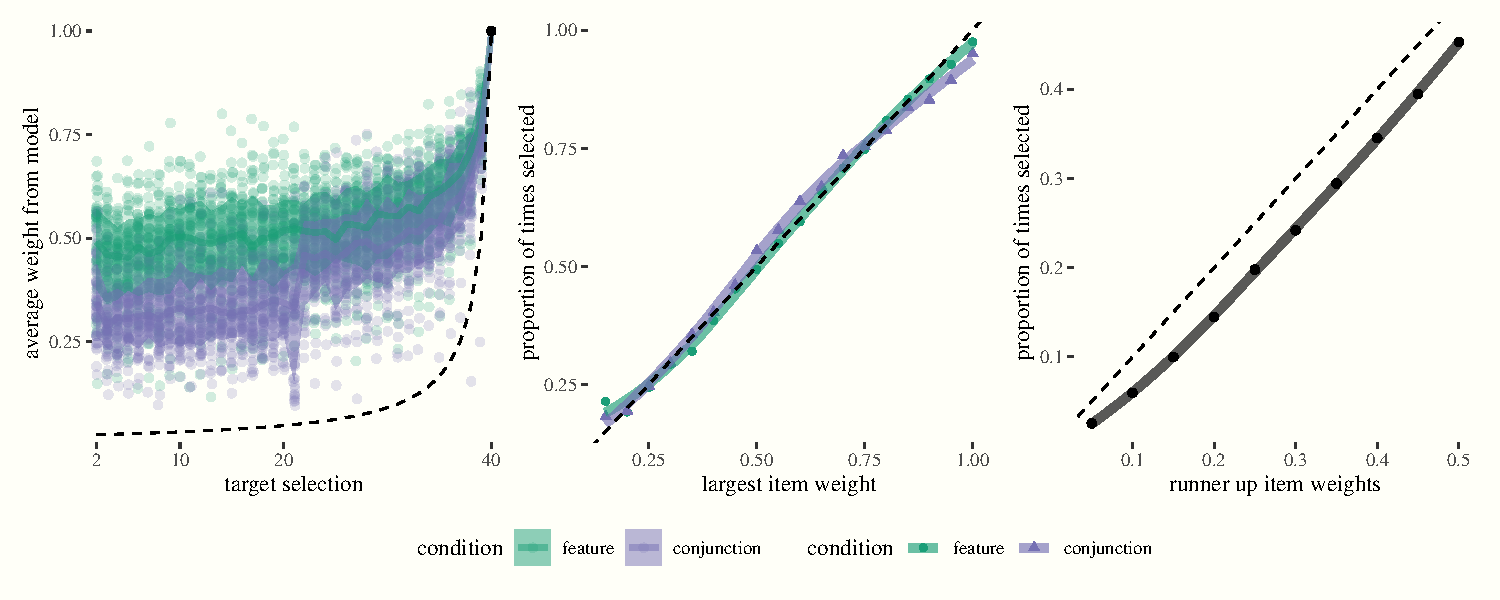
\includegraphics[width=12 cm]{Figures/qjep_preds.pdf}
\caption{(\textit{left}) Posterior probabilities for target selections during a visual foraging task. Each dot shows the  data from an individual participant, averaged over trials, in a condition and the shaded region indicates the interval in which we expect 67\% of participants to fall. The dashed line indicates chance performance. (\textit{centre})  Calibration plot for our foraging model. The $x$-axis gives the largest weight assigned by the model while the $y$-axis shows how often that target was actually selected by a human participant. (\textit{right}) This plot shows how often the 2nd and 3rd ranked items are selected based on the weights assigned by the model.}
\label{fig:cal}
\end{figure}   

Figure \ref{fig:cal2} hints at some individual differences when it comes to how predictable the model is: we can see a lot of variation in the size of the weights. However, interestingly, we find that this variability can be explained by our model parameters: nearly all of the differences between people, and between feature and conjunction conditions, can be explained by the $bP$ parameter, which is our proximity bias. The model is doing a better job with participants who show a stronger proximity bias. 

\begin{figure}[H]
\centering
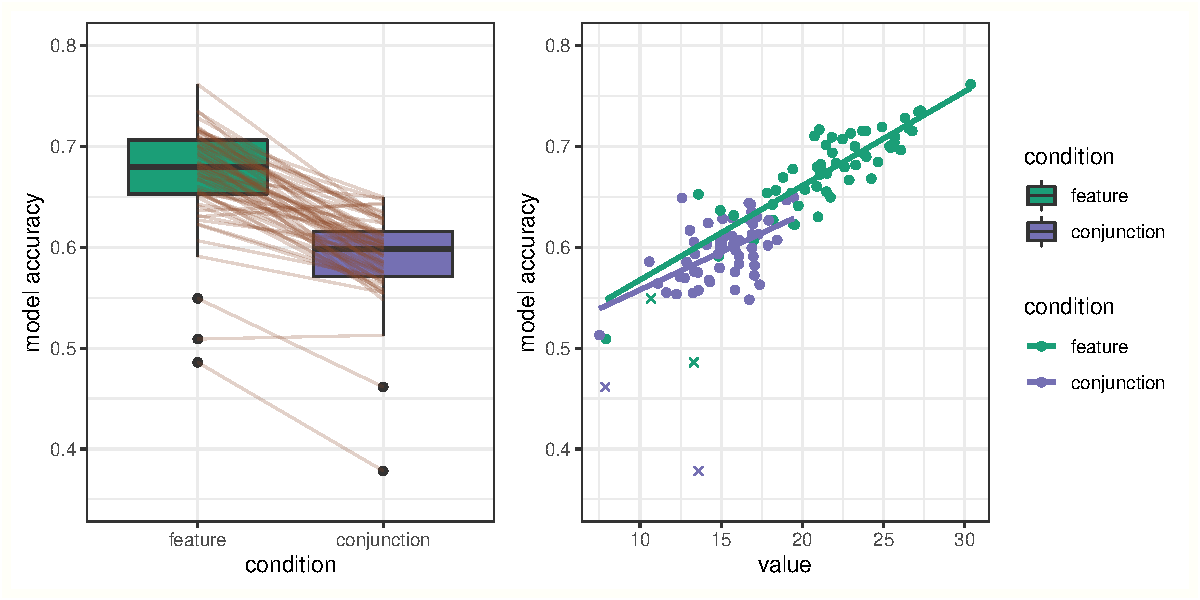
\includegraphics[width=12 cm]{Figures/qjep_indiv_diff.pdf}
\caption{(\textit{left}) Prediction scores for participants. Boxplots show quartile range and the grey lines indicate individual participants. The dots indicate outliers. (\textit{right}) Accuracy of our model varies with the strength of an individual’s \textit{bP} parameter. We can see two clear outlier participants (marked with an X).}
\label{fig:cal2}
\end{figure}   

\begin{figure}[H]
\centering
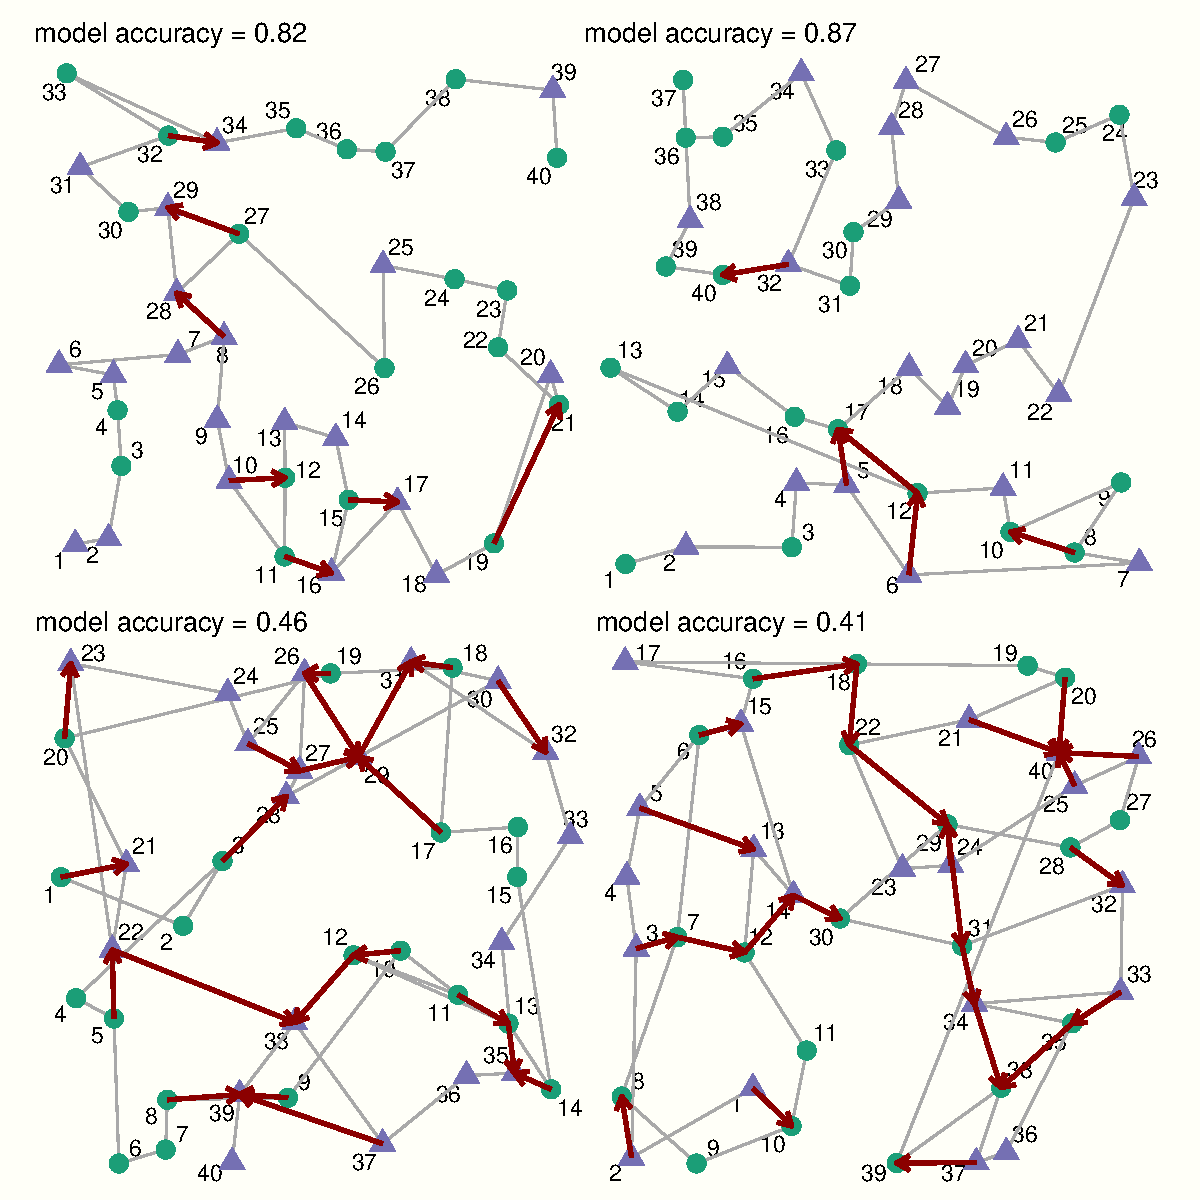
\includegraphics[width=12 cm]{Figures/qjep_ex_paths.pdf}
\caption{(\textit{top}) Two randomly selected trials in which the model does a good job in accounting for human behaviour. Red arrows indicate places where the model prediction deviates from participant behaviour. When participants diverge from the model's prediction, it appears to be due to some form of path-length optimisation. (\textit{bottom}) Two randomly selected examples in which the model does a less good job in accounting for the order in which human participants selected the items.}
\label{fig:qjep_paths}
\end{figure} 

\section{Improving the model: location of the first target selection}

One weakness of the foraging model by \cite{clarke2022foraging} is that it makes little attempt to the predict which item will be selected first. In this section we aim to improve this by modelling participant bias/preference in their choice of initial target selection. Following \cite{clarke_tatler2014, clarke2017} we fit truncated Gaussian distributions to the $(x,y)$ coordinates of the initial target selections 

\subsection{Results}

Figure \ref{fig:qjep_init_sel_hex} shows the distribution of the locations of first target selections. We can see that unlike the central bias in fixations during scene viewing, the distribution of initial target locations appear to be bimodal: while most targets are positioned in the top left hand corner <CHECK MATLAB CODE!!!> there is a second smaller distribution of central target selections. This appears to be due to different participants choosing to utilise different strategies rather than within-subject variation. However, we have no evidence that these different initial strategies affect the model parameters in any systematic way (see Supplementary Material).

\begin{figure}[H]
\centering
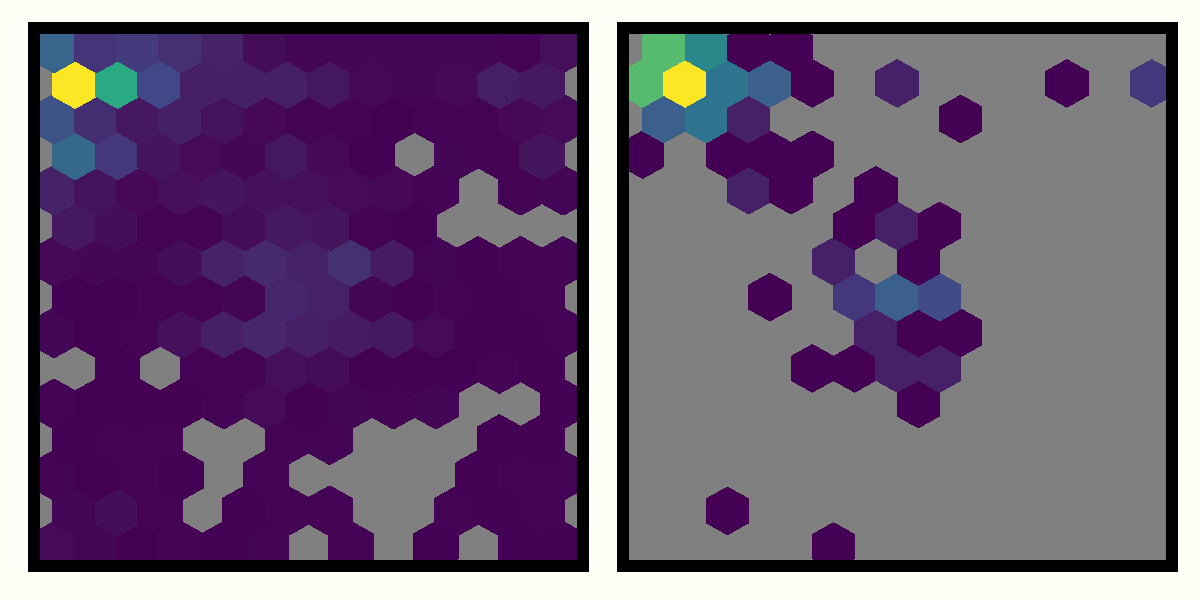
\includegraphics[width=12 cm]{Figures/init_sel_hex_plot.pdf}
\caption{Hexagonal heatmaps showing the two-dimensional distribution of the location of initial target selections. Grey areas indicate cells with a count of 0/ (\textit{left}) shows the distribution over all initial target selections while (\textit{right}) shows the distribution of each participant's median initial selection. }
\label{fig:qjep_init_sel_hex}
\end{figure} 

We modelled this bias using a multi-level two-dimensional $[0, 1]$ truncated Gaussian distribution, the results of which are shown in Figure \ref{fig:qjep_init_sel_mdl}\footnote{Full details of the analysis can be found in the supplementary materials}.

\begin{figure}[H]
\centering
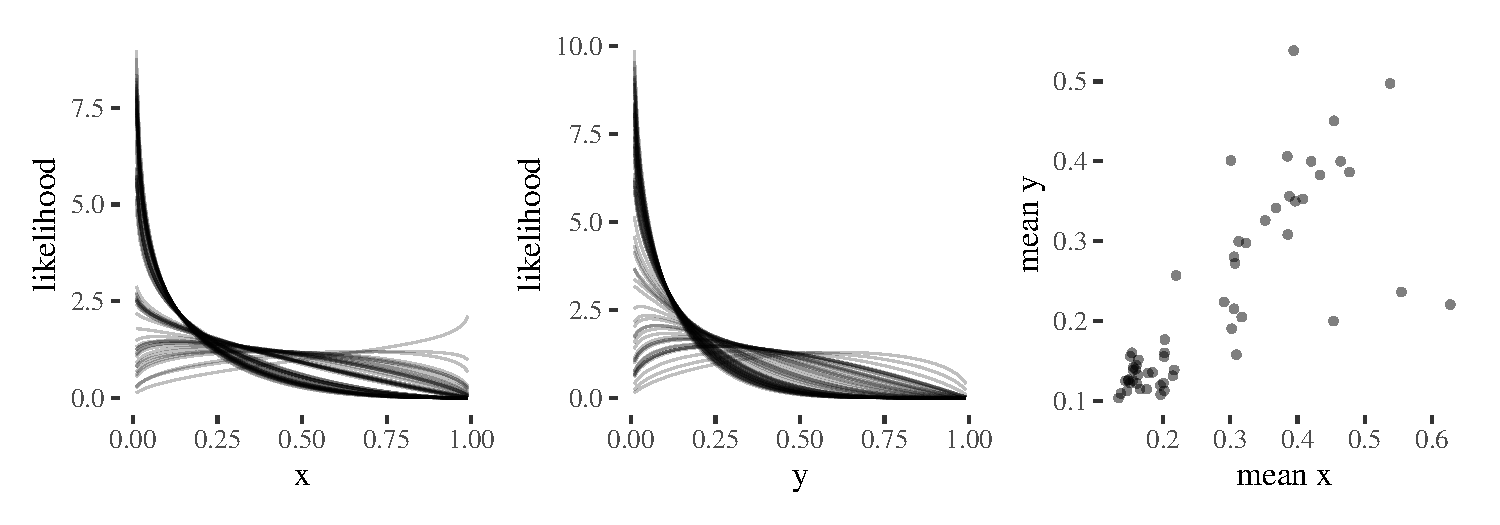
\includegraphics[width=12 cm]{Figures/init_sel_mdl.pdf}
\caption{Posterior fits for (\textit{left}) horizontal and (\textit{middle}) vertical locations of the initial target selection. Each line represents a different participant.  (\textit{right}) shows the correlation between participant's mean $x$ and $y$ coordinates. The box shows the extent of the stimulus.}
\label{fig:qjep_init_sel_mdl}
\end{figure} 



\subsection{Figures, Tables and Schemes}

All figures and tables should be cited in the main text as Figure~\ref{fig1}, Table~\ref{tab1}, Table~\ref{tab2}, etc.


\unskip

\begin{table}[H] 
\caption{This is a table caption. Tables should be placed in the main text near to the first time they are~cited.\label{tab1}}
\newcolumntype{C}{>{\centering\arraybackslash}X}
\begin{tabularx}{\textwidth}{CCC}
\toprule
\textbf{Title 1}	& \textbf{Title 2}	& \textbf{Title 3}\\
\midrule
Entry 1		& Data			& Data\\
Entry 2		& Data			& Data\\
\bottomrule
\end{tabularx}
\end{table}
\unskip

\begin{table}[H]
\caption{This is a wide table.\label{tab2}}
	\begin{adjustwidth}{-\extralength}{0cm}
		\newcolumntype{C}{>{\centering\arraybackslash}X}
		\begin{tabularx}{\fulllength}{CCCC}
			\toprule
			\textbf{Title 1}	& \textbf{Title 2}	& \textbf{Title 3}     & \textbf{Title 4}\\
			\midrule
			Entry 1		& Data			& Data			& Data\\
			Entry 2		& Data			& Data			& Data\textsuperscript{1}\\
			\bottomrule
		\end{tabularx}
	\end{adjustwidth}
	\noindent{\footnotesize{\textsuperscript{1} This is a table footnote.}}
\end{table}

%\begin{listing}[H]
%\caption{Title of the listing}
%\rule{\columnwidth}{1pt}
%\raggedright Text of the listing. In font size footnotesize, small, or normalsize. Preferred format: left aligned and single spaced. Preferred border format: top border line and bottom border line.
%\rule{\columnwidth}{1pt}
%\end{listing}

Text.

Text.

\subsection{Formatting of Mathematical Components}

This is the example 1 of equation:
\begin{linenomath}
\begin{equation}
a = 1,
\end{equation}
\end{linenomath}
the text following an equation need not be a new paragraph. Please punctuate equations as regular text.
%% If the documentclass option "submit" is chosen, please insert a blank line before and after any math environment (equation and eqnarray environments). This ensures correct linenumbering. The blank line should be removed when the documentclass option is changed to "accept" because the text following an equation should not be a new paragraph.


% Example of a page in landscape format (with table and table footnote).
%\startlandscape
%\begin{table}[H] %% Table in wide page
%\caption{This is a very wide table.\label{tab3}}
%	\begin{tabularx}{\textwidth}{CCCC}
%		\toprule
%		\textbf{Title 1}	& \textbf{Title 2}	& \textbf{Title 3}	& \textbf{Title 4}\\
%		\midrule
%		Entry 1		& Data			& Data			& This cell has some longer content that runs over two lines.\\
%		Entry 2		& Data			& Data			& Data\textsuperscript{1}\\
%		\bottomrule
%	\end{tabularx}
%	\begin{adjustwidth}{+\extralength}{0cm}
%		\noindent\footnotesize{\textsuperscript{1} This is a table footnote.}
%	\end{adjustwidth}
%\end{table}
%\finishlandscape

% Example of a figure that spans the whole page width. The same concept works for tables, too.
\begin{figure}[H]
\begin{adjustwidth}{-\extralength}{0cm}
\centering

\includegraphics[width=15cm]{Definitions/logo-mdpi}
\end{adjustwidth}
\caption{This is a wide figure.\label{fig2}}
\end{figure}  

Please punctuate equations as regular text. Theorem-type environments (including propositions, lemmas, corollaries etc.) can be formatted as follows:
%% Example of a theorem:
\begin{Theorem}
Example text of a theorem.
\end{Theorem}

The text continues here. Proofs must be formatted as follows:

%% Example of a proof:
\begin{proof}[Proof of Theorem 1]
Text of the proof. Note that the phrase ``of Theorem 1'' is optional if it is clear which theorem is being referred to.
\end{proof}
The text continues here.

%%%%%%%%%%%%%%%%%%%%%%%%%%%%%%%%%%%%%%%%%%
\section{Discussion}

Authors should discuss the results and how they can be interpreted from the perspective of previous studies and of the working hypotheses. The findings and their implications should be discussed in the broadest context possible. Future research directions may also be highlighted.

Remaining open questions

%%%%%%%%%%%%%%%%%%%%%%%%%%%%%%%%%%%%%%%%%%
\vspace{6pt} 

%%%%%%%%%%%%%%%%%%%%%%%%%%%%%%%%%%%%%%%%%%
%% optional
%\supplementary{The following are available online at \linksupplementary{s1}, Figure S1: title, Table S1: title, Video S1: title.}

% Only for the journal Methods and Protocols:
% If you wish to submit a video article, please do so with any other supplementary material.
% \supplementary{The following are available at \linksupplementary{s1}, Figure S1: title, Table S1: title, Video S1: title. A supporting video article is available at doi: link.} 

%%%%%%%%%%%%%%%%%%%%%%%%%%%%%%%%%%%%%%%%%%
\authorcontributions{For research articles with several authors, a short paragraph specifying their individual contributions must be provided. The following statements should be used ``Conceptualization, X.X. and Y.Y.; methodology, X.X.; software, X.X.; validation, X.X., Y.Y. and Z.Z.; formal analysis, X.X.; investigation, X.X.; resources, X.X.; data curation, X.X.; writing---original draft preparation, X.X.; writing---review and editing, X.X.; visualization, X.X.; supervision, X.X.; project administration, X.X.; funding acquisition, Y.Y. All authors have read and agreed to the published version of the manuscript.'', please turn to the  \href{http://img.mdpi.org/data/contributor-role-instruction.pdf}{CRediT taxonomy} for the term explanation. Authorship must be limited to those who have contributed substantially to the work~reported.}

\funding{Please add: ``This research received no external funding'' or ``This research was funded by NAME OF FUNDER grant number XXX.'' and  and ``The APC was funded by XXX''. Check carefully that the details given are accurate and use the standard spelling of funding agency names at \url{https://search.crossref.org/funding}, any errors may affect your future funding.}

\institutionalreview{In this section, please add the Institutional Review Board Statement and approval number for studies involving humans or animals. Please note that the Editorial Office might ask you for further information. Please add ``The study was conducted according to the guidelines of the Declaration of Helsinki, and approved by the Institutional Review Board (or Ethics Committee) of NAME OF INSTITUTE (protocol code XXX and date of approval).'' OR ``Ethical review and approval were waived for this study, due to REASON (please provide a detailed justification).'' OR ``Not applicable'' for studies not involving humans or animals. You might also choose to exclude this statement if the study did not involve humans or animals.}

\informedconsent{Any research article describing a study involving humans should contain this statement. Please add ``Informed consent was obtained from all subjects involved in the study.'' OR ``Patient consent was waived due to REASON (please provide a detailed justification).'' OR ``Not applicable'' for studies not involving humans. You might also choose to exclude this statement if the study did not involve humans.

Written informed consent for publication must be obtained from participating patients who can be identified (including by the patients themselves). Please state ``Written informed consent has been obtained from the patient(s) to publish this paper'' if applicable.}

\dataavailability{In this section, please provide details regarding where data supporting reported results can be found, including links to publicly archived datasets analyzed or generated during the study. Please refer to suggested Data Availability Statements in section ``MDPI Research Data Policies'' at \url{https://www.mdpi.com/ethics}. You might choose to exclude this statement if the study did not report any data.} 

\acknowledgments{In this section you can acknowledge any support given which is not covered by the author contribution or funding sections. This may include administrative and technical support, or donations in kind (e.g., materials used for experiments).}

\conflictsofinterest{Declare conflicts of interest or state ``The authors declare no conflict of interest.'' Authors must identify and declare any personal circumstances or interest that may be perceived as inappropriately influencing the representation or interpretation of reported research results. Any role of the funders in the design of the study; in the collection, analyses or interpretation of data; in the writing of the manuscript, or in the decision to publish the results must be declared in this section. If there is no role, please state ``The funders had no role in the design of the study; in the collection, analyses, or interpretation of data; in the writing of the manuscript, or in the decision to publish the~results''.} 

%%%%%%%%%%%%%%%%%%%%%%%%%%%%%%%%%%%%%%%%%%
%% Only for journal Encyclopedia
%\entrylink{The Link to this entry published on the encyclopedia platform.}

%%%%%%%%%%%%%%%%%%%%%%%%%%%%%%%%%%%%%%%%%%
%% Optional
\abbreviations{Abbreviations}{
The following abbreviations are used in this manuscript:\\

\noindent 
\begin{tabular}{@{}ll}
MDPI & Multidisciplinary Digital Publishing Institute\\
DOAJ & Directory of open access journals\\
TLA & Three letter acronym\\
LD & Linear dichroism
\end{tabular}}

%%%%%%%%%%%%%%%%%%%%%%%%%%%%%%%%%%%%%%%%%%
%% Optional
\appendixtitles{no} % Leave argument "no" if all appendix headings stay EMPTY (then no dot is printed after "Appendix A"). If the appendix sections contain a heading then change the argument to "yes".
\appendixstart
\appendix
\section[\appendixname~\thesection]{}
\subsection[\appendixname~\thesubsection]{}
The appendix is an optional section that can contain details and data supplemental to the main text---for example, explanations of experimental details that would disrupt the flow of the main text but nonetheless remain crucial to understanding and reproducing the research shown; figures of replicates for experiments of which representative data are shown in the main text can be added here if brief, or as Supplementary Data. Mathematical proofs of results not central to the paper can be added as an appendix.

\begin{table}[H] 
\caption{This is a table caption.\label{tab5}}
\newcolumntype{C}{>{\centering\arraybackslash}X}
\begin{tabularx}{\textwidth}{CCC}
\toprule
\textbf{Title 1}	& \textbf{Title 2}	& \textbf{Title 3}\\
\midrule
Entry 1		& Data			& Data\\
Entry 2		& Data			& Data\\
\bottomrule
\end{tabularx}
\end{table}

\section[\appendixname~\thesection]{}
All appendix sections must be cited in the main text. In the appendices, Figures, Tables, etc. should be labeled, starting with ``A''---e.g., Figure A1, Figure A2, etc.

%%%%%%%%%%%%%%%%%%%%%%%%%%%%%%%%%%%%%%%%%%
\begin{adjustwidth}{-\extralength}{0cm}
%\printendnotes[custom] % Un-comment to print a list of endnotes

\reftitle{References}

%=====================================
% References, variant A: external bibliography
%=====================================
\bibliography{literature.bib}

\end{adjustwidth}
\end{document}

